\documentclass[12pt]{article}

% --- Preámbulo ---
\usepackage[utf8]{inputenc}
\usepackage[T1]{fontenc}
\usepackage[spanish,es-noshorthands,es-tabla]{babel}
\usepackage{amsmath, amssymb}
\usepackage{graphicx}
\usepackage{booktabs}
\usepackage{geometry}
\geometry{margin=2cm}
\usepackage{xcolor}
\usepackage{float}
\usepackage{hyperref}
\hypersetup{
    colorlinks=true,
    linkcolor=blue,
    citecolor=blue,
    filecolor=magenta,
    urlcolor=cyan,
    pdftitle={Detección de cambios satelital -- Sismo de San José del Palmar 2026}
}
\usepackage{csquotes}
\usepackage[backend=biber, style=authoryear]{biblatex}
\addbibresource{references.bib}

% \fig[ancho]{archivo}{pie de figura}{etiqueta}: incluye la figura si existe; si no, muestra un recuadro.
\newcommand{\fig}[4][0.8]{%
  \begin{figure}[H]
    \centering
    \IfFileExists{figures/#2}{%
      \includegraphics[width=#1\textwidth]{figures/#2}%
    }{%
      \fbox{\parbox[c][4cm][c]{0.7\textwidth}{\centering\textcolor{red}{Falta la figura: figures/#2}}}%
    }
    \caption{#3}
    \label{#4}
  \end{figure}}

% --- Metadatos ---
\title{Proyecto de Medio Semestre: Cartografía de deslizamientos cosísmicos del sismo $M_w$~7.4 de San José del Palmar (Chocó, Colombia) del 10 de agosto de 2026 mediante $\Delta$NDVI de Sentinel-2}
\author{Jorge Sierra \and Hania Valentina Carreño \and Andrés Felipe Barrios Bohórquez \and Nicolás León Parra}
\date{\today}

\begin{document}

\maketitle

\begin{abstract}
El 10 de agosto de 2026 a las 12:34~UTC, un sismo de magnitud $M_w$~7.4 y profundidad intermedia ($\sim$110~km), con epicentro cerca de San José del Palmar (Chocó), sacudió el occidente y centro de Colombia, detonando movimientos en masa a lo largo de la Cordillera Occidental y dañando infraestructura urbana en Pereira, Manizales y Cali. Este informe documenta un flujo de trabajo reproducible de detección de cambios bitemporal, implementado en QGIS, para cartografiar los deslizamientos cosísmicos en un área de $\sim$50~km$^2$ del cañón del río Ingará, alrededor de San José del Palmar. Se utilizaron imágenes Sentinel-2 Nivel-2A (reflectancia de superficie, BOA) del 24 de julio de 2026 ($t_1$) y del 18 de agosto de 2026 ($t_2$), corregistradas en una grilla común de 10~m en MAGNA-SIRGAS Origen Nacional (EPSG:9377), enmascaradas de nubes con la capa de clasificación de escena (SCL) y comparadas mediante la diferencia de NDVI ($\Delta$NDVI) y la diferencia de la banda del infrarrojo cercano ($\Delta$NIR). Un umbral $\mu - 2\sigma$ sobre el $\Delta$NDVI identificó 181 polígonos candidatos a deslizamiento que suman 95.2~ha (1.9\% del área de estudio), el mayor de ellos de 6.0~ha.
\end{abstract}

% =====================================================================
\section{Introducción}
Los sismos en terrenos montañosos rara vez actúan solos: al movimiento del terreno le siguen, en segundos o días, cientos o miles de fallas de ladera que sepultan vías, represan ríos y aíslan comunidades. En Colombia, donde los Andes se dividen en tres cordilleras con pendientes fuertes, suelos residuales profundos y alta precipitación, los deslizamientos cosísmicos son uno de los efectos secundarios más dañinos de los eventos sísmicos. Su cartografía rápida y objetiva es por lo tanto esencial para la atención de la emergencia (rutas de acceso, poblaciones aisladas) y para la gestión del riesgo a largo plazo.

Las imágenes satelitales ópticas permiten detectar deslizamientos de forma directa, ya que una falla de ladera remueve la cobertura vegetal y expone suelo y roca, lo que produce una caída marcada en índices de vegetación como el Índice de Vegetación de Diferencia Normalizada (NDVI) \parencite{Tucker1979}. Comparar imágenes adquiridas antes ($t_1$) y después ($t_2$) del evento permite aislar estos cambios del fondo estable \parencite{Lillesand2015}.

Este proyecto aplica dicho principio al sismo $M_w$~7.4 del 10 de agosto de 2026 con epicentro cerca de San José del Palmar (Chocó). Los objetivos específicos son:
\begin{itemize}
    \item Adquirir y preprocesar un par de imágenes Sentinel-2 L2A radiométricamente comparables que enmarquen el evento.
    \item Calcular índices espectrales (NDVI) y diferencias de imágenes ($\Delta$NDVI, $\Delta$NIR) para resaltar la pérdida de vegetación.
    \item Separar el cambio real del ruido mediante un umbral estadístico, vectorizar el resultado y cuantificar el área afectada.
\end{itemize}

% =====================================================================
\section{Región de Interés (ROI) y caso de estudio}
\subsection{El evento}
Según el Servicio Geológico Colombiano \parencite{SGC2026}, el sismo ocurrió el 10 de agosto de 2026 a las 07:34 hora local (12:34~UTC), con magnitud $M_w$~7.4 y una profundidad hipocentral cercana a 110~km, lo que lo convierte en el sismo más fuerte registrado en Colombia en la última década. Su profundidad intermedia explica por qué la sacudida fuerte se sintió en un área muy amplia, desde el Chocó hasta el Eje Cafetero y el Valle del Cauca. El Gobierno nacional declaró la situación de desastre nacional; las cifras reportadas alcanzaron varios centenares de fallecidos, miles de heridos y daños extensos en viviendas, hospitales, vías y aeropuertos \parencite{ReliefWeb2026}. El Servicio de Gestión de Emergencias de Copernicus activó el mapeo rápido (EMSR916) sobre siete áreas de interés, incluida Pereira \parencite{CEMS_EMSR916}. Las vías de acceso a San José del Palmar fueron reportadas bloqueadas o sepultadas por deslizamientos, dejando aislado al municipio.

\subsection{Área de estudio}
La ROI (Figura~\ref{fig:location}) es un polígono de 49.7~km$^2$ (497\,321 píxeles de 10~m) en la vertiente pacífica de la Cordillera Occidental, que cubre el cañón del río Ingará, los asentamientos rurales de La Italia, La Lomita, La Badea y San Pedro de Ingará, y el casco urbano de San José del Palmar (4.90$^\circ$N, 76.23$^\circ$W). El terreno es empinado y profundamente disectado, cubierto por bosque húmedo tropical y subandino mezclado con pastos y pequeñas fincas, lo que lo hace muy susceptible a deslizamientos superficiales. La ROI se dibujó en el Copernicus Browser evitando la nubosidad persistente y se almacenó como GeoPackage (\texttt{roi.gpkg}, capa \texttt{roi\_palmar}) en EPSG:9377.

\fig{fig_location.jpg}{Localización del área de estudio (ROI) alrededor de San José del Palmar, Chocó, Colombia. Límites departamentales: GADM.}{fig:location}

% =====================================================================
\section{Metodología}
La implementación sigue un flujo de trabajo estructurado \parencite{Lillesand2015} desarrollado íntegramente en QGIS~3.44 \parencite{QGIS_Software}, utilizando el Copernicus Browser para la adquisición de datos y las herramientas de QGIS \emph{Align Rasters}, \emph{Raster Calculator}, \emph{Translate}, \emph{Raster layer statistics}, \emph{Sieve}, \emph{Polygonize}, \emph{Field Calculator} y \emph{Print Layout} para el procesamiento, la cuantificación y la cartografía. El flujo tiene cuatro fases: (1) definición del problema y adquisición de datos, (2) preprocesamiento, (3) procesamiento y análisis de imágenes, y (4) posprocesamiento y evaluación de exactitud.

\subsection{Fase 1: Definición del problema y adquisición de datos}
\begin{itemize}
    \item \textbf{Fechas:} La ROI presenta nubosidad persistente, por lo que se inspeccionaron visualmente todas las adquisiciones Sentinel-2 L2A entre junio y septiembre de 2026. La imagen \emph{antes} ($t_1$) es la del \textbf{24 de julio de 2026}, la adquisición casi libre de nubes más cercana antes del evento (17 días antes). El paso de Sentinel-2 del 10 de agosto de 2026 ($\sim$15:20~UTC) ocurrió unas tres horas \emph{después} del sismo, pero la ROI estaba cubierta de nubes; por ello se seleccionó como $t_2$ la primera adquisición despejada posterior, el \textbf{18 de agosto de 2026} (8 días después). Ambas fechas pertenecen a la misma temporada, lo que minimiza las diferencias fenológicas.
    \item \textbf{Fuentes de datos:} Sentinel-2 MSI Nivel-2A \parencite{ESA2023}, descargado del Copernicus Data Space Ecosystem (Copernicus Browser, descarga \emph{Analytical}) \parencite{CDSE}, recortado a la ROI, como GeoTIFF de reflectancia en punto flotante de 32 bits, en UTM 18N (EPSG:32618) a 10~m. Capas descargadas: B02 (azul), B03 (verde), B04 (rojo), B08 (infrarrojo cercano, NIR), B11 y B12 (infrarrojo de onda corta, SWIR), el mapa de clasificación de escena (SCL) y los compuestos en color verdadero y falso color.
\end{itemize}

\paragraph{Selección de fechas y del área de estudio.} Inicialmente se evaluó como imagen \emph{antes} la escena del \textbf{14 de julio de 2026}, la de menor nubosidad de ese mes (Figura~\ref{fig:cap_14jul}), comparada con la escena del 18 de agosto sobre el casco urbano (Figura~\ref{fig:cap_18ago}). Se ensayaron varias delimitaciones de la ROI bordeando las nubes (Figuras~\ref{fig:cap_aoi_14jul}, \ref{fig:cap_aoi_op1} y~\ref{fig:cap_aoi_op2}): la primera era demasiado pequeña ($\sim$6--15~km$^2$) y abarcaba poco más que el casco urbano, por lo que se amplió hacia el oeste para incluir el cañón del río Ingará, donde se esperan los deslizamientos. Con el área ampliada, la escena del \textbf{24 de julio de 2026} resultó más limpia sobre la ROI y más cercana al evento que la del 14 de julio, por lo que se adoptó como $t_1$ definitiva.

\fig[0.85]{cap_t1_14jul_zoom.jpg}{Copernicus Browser: escena Sentinel-2 L2A del 14 de julio de 2026 sobre San José del Palmar (primera candidata a imagen \emph{antes}).}{fig:cap_14jul}
\fig[0.85]{cap_t2_18ago_zoom.jpg}{Copernicus Browser: escena Sentinel-2 L2A del 18 de agosto de 2026 sobre San José del Palmar (imagen \emph{después}).}{fig:cap_18ago}
\fig[0.85]{cap_aoi_14jul.jpg}{Primera delimitación de la ROI sobre la escena del 14 de julio de 2026, bordeando las nubes.}{fig:cap_aoi_14jul}
\fig[0.75]{cap_aoi_opcion1.jpg}{Segunda delimitación de la ROI, ampliada hacia el cañón del río Ingará.}{fig:cap_aoi_op1}
\fig[0.85]{cap_aoi_opcion2.jpg}{Tercera delimitación de la ROI, con mayor amplitud para cubrir las laderas del cañón.}{fig:cap_aoi_op2}

La Figura~\ref{fig:cap_aoi_t1} muestra la ROI final (49.5~km$^2$) dibujada en el Copernicus Browser sobre la imagen del 24 de julio, bordeando las nubes, y la Figura~\ref{fig:cap_aoi_t2} la misma área el 18 de agosto, completamente despejada. Las Figuras~\ref{fig:cap_descarga} y~\ref{fig:cap_descarga_t2} muestran la configuración de la descarga \emph{Analytical} para cada fecha.

\fig[0.85]{cap_aoi_t1.jpg}{ROI dibujada en el Copernicus Browser sobre la escena Sentinel-2 L2A del 24 de julio de 2026 ($t_1$).}{fig:cap_aoi_t1}
\fig[0.85]{cap_aoi_t2.jpg}{Escena Sentinel-2 L2A del 18 de agosto de 2026 ($t_2$) en el Copernicus Browser: la zona de estudio aparece libre de nubes.}{fig:cap_aoi_t2}
\fig[0.95]{cap_descarga.jpg}{Configuración de la descarga \emph{Analytical} en el Copernicus Browser: TIFF de 32 bits, resolución personalizada de 10~m, UTM 18N (EPSG:32618), bandas crudas B02, B03, B04, B08, B11, B12, compuestos en color verdadero y falso color y mapa de clasificación de escena, recortados a la ROI (fecha 24 de julio de 2026).}{fig:cap_descarga}
\fig[0.95]{cap_descarga_t2.jpg}{Descarga \emph{Analytical} con la misma configuración para la fecha 18 de agosto de 2026.}{fig:cap_descarga_t2}

\begin{table}[H]
    \centering
    \caption{Escenas Sentinel-2 utilizadas en el estudio.}
    \label{tab:scenes}
    \begin{tabular}{llll}
        \toprule
        \textbf{Rol} & \textbf{Fecha} & \textbf{Producto / Nivel} & \textbf{Área enmascarada en la ROI} \\
        \midrule
        $t_1$ (antes)   & 2026-07-24 & Sentinel-2 MSI L2A & 2.4\% \\
        $t_2$ (después) & 2026-08-18 & Sentinel-2 MSI L2A & 3.1\% (cirros delgados) \\
        \bottomrule
    \end{tabular}
\end{table}

\subsection{Fase 2: Preprocesamiento}
Para garantizar que las imágenes fueran radiométricamente comparables se aplicaron los siguientes pasos:
\begin{itemize}
    \item \textbf{Corrección atmosférica:} Se usaron productos de Nivel-2A, ya corregidos a reflectancia de superficie (BOA) por el procesador Sen2Cor de la ESA \parencite{Main-Knorn2017}. Los valores son reflectancias entre 0 y 1 (p.~ej., NIR B08 medio $\approx$ 0.25 y rojo B04 $\approx$ 0.02 sobre la ROI), y la mediana del NDVI de los píxeles clasificados como vegetación fue 0.87 tanto en $t_1$ como en $t_2$, típica de bosque tropical denso, lo que confirma que ambas fechas son radiométricamente comparables.
    \item \textbf{Corregistro:} Todas las bandas de ambas fechas se procesaron con la herramienta \emph{Align Rasters} de QGIS, usando la banda B04 de $t_1$ como capa de referencia y reproyectando a EPSG:9377 sobre una grilla idéntica de 10~m (mismo origen, 1054 $\times$ 681 píxeles). La alineación se verificó visualmente alternando los compuestos en color verdadero de $t_1$ y $t_2$ sobre cruces de vías y curvas del río, sin desplazamientos visibles (subpíxel, en concordancia con la especificación de corregistro multitemporal de Sentinel-2) (Figuras~\ref{fig:cap_align}, \ref{fig:cap_b12} y~\ref{fig:coreg}).
    \item \textbf{Remuestreo:} Las bandas se remuestrearon por interpolación bilineal y la capa SCL por vecino más cercano, para preservar los valores de clase. Se desactivó la opción \emph{``rescale values according to cell size''} para no alterar las reflectancias. Así, las bandas de 20~m (B11, B12, SCL) quedaron en la grilla común de 10~m.
    \item \textbf{Enmascaramiento de nubes:} Se usó como banda de calidad la capa de clasificación de escena (SCL) de Sen2Cor. Como se descargó en la visualización RGB estándar de Sentinel Hub, las clases se decodificaron a partir de sus colores fijos en la Calculadora Ráster, y se enmascararon los píxeles clasificados como sin dato (0), sombra de nube (3), nube de probabilidad media (8), nube de probabilidad alta (9) y cirros delgados (10). La máscara común se obtuvo como $valid = clear_{t_1} \times clear_{t_2}$ (Figura~\ref{fig:mask}); el 95.2\% de la ROI quedó válido. En $t_1$ se enmascaró el 2.4\% de la ROI (principalmente sombra de nube, 1.5\%) y en $t_2$ el 3.1\%, en su mayoría píxeles marcados como cirros delgados (2.3\%).
\end{itemize}

\paragraph{Preprocesamiento en QGIS.} Las bandas descargadas se cargaron en un proyecto de QGIS en EPSG:9377 (Figura~\ref{fig:cap_qgis}) y se renombraron con una nomenclatura corta por fecha (\texttt{t1\_B04}, \texttt{t2\_B08}, etc.; Figura~\ref{fig:cap_renombrar}). La ROI se guardó como GeoPackage (Figura~\ref{fig:cap_roi}). Luego se ejecutó \emph{Align Rasters} (Figuras~\ref{fig:cap_align} y~\ref{fig:cap_align_run}), que generó el grupo de capas alineadas (Figura~\ref{fig:cap_aligned}); finalmente se retiraron del proyecto las bandas originales sin alinear para evitar confusiones de nombres en la Calculadora Ráster, conservando solo los compuestos de color para visualización (Figura~\ref{fig:cap_final}).

\fig[0.95]{cap_qgis_capas.jpg}{Bandas descargadas de ambas fechas cargadas en QGIS (proyecto en EPSG:9377).}{fig:cap_qgis}
\fig[0.6]{cap_qgis_renombrar.jpg}{Capas renombradas por fecha y banda en el panel de capas de QGIS.}{fig:cap_renombrar}
\fig[0.45]{cap_qgis_roi.jpg}{ROI almacenada como GeoPackage (\texttt{layername=roi\_palmar}) junto a las bandas de $t_1$.}{fig:cap_roi}
\fig[0.8]{cap_align.jpg}{Configuración por capa en \emph{Align Rasters}: remuestreo bilineal para las bandas y vecino más cercano para el mapa de clasificación de escena.}{fig:cap_align}
\fig[0.8]{cap_align_run.jpg}{Parámetros generales de \emph{Align Rasters}: 14 capas de entrada, capa de referencia \texttt{t1\_B04}, CRS EPSG:9377 (MAGNA-SIRGAS Origen Nacional) y tamaño de celda de 10~m.}{fig:cap_align_run}
\fig[0.4]{cap_qgis_aligned.jpg}{Grupo de capas alineadas (\texttt{alligned}) resultante para ambas fechas.}{fig:cap_aligned}
\fig[0.4]{cap_qgis_final.jpg}{Organización final del proyecto QGIS: compuestos de color originales para visualización y bandas alineadas para el análisis.}{fig:cap_final}

\begin{figure}[H]
  \centering
  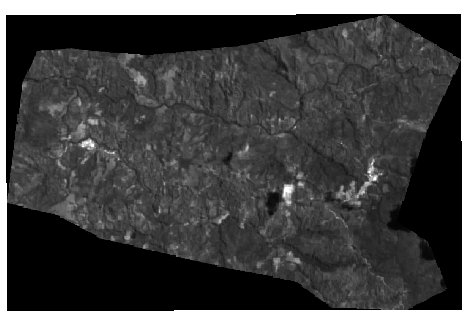
\includegraphics[width=0.45\textwidth]{figures/cap_b12_t1.jpg}\hfill
  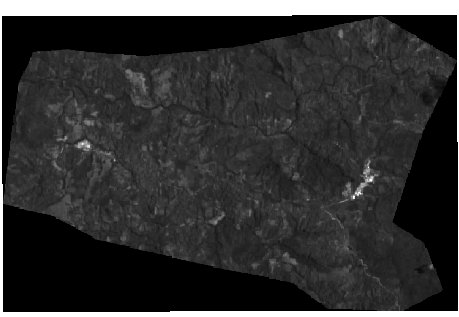
\includegraphics[width=0.45\textwidth]{figures/cap_b12_t2.jpg}
  \caption{Banda B12 (SWIR) ya alineada en QGIS: $t_1$ (izquierda, con algo de nubosidad) y $t_2$ (derecha, despejada).}
  \label{fig:cap_b12}
\end{figure}

\fig[0.9]{fig_coregistration.jpg}{Verificación visual del corregistro entre $t_1$ y $t_2$ (casco urbano de San José del Palmar; las líneas cian marcan el mismo punto en ambas fechas).}{fig:coreg}
\fig[0.6]{fig_mask.jpg}{Máscara común de píxeles válidos (blanco = despejado en ambas fechas; negro = nube, sombra, cirro o sin dato en al menos una fecha).}{fig:mask}

\subsection{Fase 3: Procesamiento y análisis de imágenes}
Se aplicaron dos técnicas complementarias de detección de cambios (Tabla~\ref{tab:techniques}).

\begin{table}[H]
    \centering
    \caption{Metodologías de detección de cambios aplicadas.}
    \label{tab:techniques}
    \begin{tabular}{p{3.4cm}p{11.3cm}}
        \toprule
        \textbf{Método} & \textbf{Técnica} \\
        \midrule
        Índices espectrales ($\Delta$NDVI) & $NDVI = \dfrac{B08 - B04}{B08 + B04}$ calculado para $t_1$ y $t_2$; $\Delta NDVI = NDVI_{t_2} - NDVI_{t_1}$. Los deslizamientos aparecen como valores fuertemente negativos (ladera vegetada $\rightarrow$ suelo desnudo). \\[2mm]
        Diferencia de imágenes ($\Delta$NIR) & $\Delta NIR = B08_{t_2} - B08_{t_1}$. La pérdida del dosel sano reduce la reflectancia en el infrarrojo cercano, resaltando cambios de gran magnitud. \\
        \bottomrule
    \end{tabular}
\end{table}

Todas las operaciones se realizaron con la Calculadora Ráster, asignando a los píxeles no válidos el valor NoData ($-9999$):
\[
\Delta NDVI =
\begin{cases}
NDVI_{t_2} - NDVI_{t_1} & \text{si } valid = 1\\
\text{NoData} & \text{en otro caso}
\end{cases}
\]

\fig[0.75]{fig_t1_truecolor.jpg}{Compuesto en color verdadero (B4-B3-B2), $t_1$ = 24 de julio de 2026.}{fig:t1tc}
\fig[0.75]{fig_t2_truecolor.jpg}{Compuesto en color verdadero (B4-B3-B2), $t_2$ = 18 de agosto de 2026. Se observan nuevas cicatrices de suelo desnudo en las laderas del cañón.}{fig:t2tc}
\fig[0.75]{fig_t1_falsecolor.jpg}{Compuesto en falso color (B8-B4-B3), $t_1$. La vegetación sana aparece en tonos rojos y el suelo desnudo en tonos cian/grises.}{fig:t1fc}
\fig[0.75]{fig_t2_falsecolor.jpg}{Compuesto en falso color (B8-B4-B3), $t_2$.}{fig:t2fc}
\fig[0.75]{fig_t1_ndvi.jpg}{NDVI en $t_1$ (24 de julio de 2026).}{fig:ndvi1}
\fig[0.75]{fig_t2_ndvi.jpg}{NDVI en $t_2$ (18 de agosto de 2026).}{fig:ndvi2}
\fig{fig_dndvi.jpg}{$\Delta$NDVI ($t_2 - t_1$). Rojo: pérdida de vegetación (deslizamientos candidatos); amarillo: sin cambio; verde: ganancia de vegetación.}{fig:dndvi}
\fig{fig_dnir.jpg}{$\Delta$NIR (B08$_{t_2}$ $-$ B08$_{t_1}$).}{fig:dnir}

% =====================================================================
\subsection{Fase 4: Posprocesamiento y evaluación de exactitud}
\begin{itemize}
    \item \textbf{Umbral:} Las estadísticas del ráster $\Delta$NDVI sobre los píxeles válidos fueron $\mu = -0.0075$ y $\sigma = 0.0467$ (rango de $-0.62$ a $+0.66$; Figura~\ref{fig:hist}). Siguiendo la regla de $\pm 2\sigma$, los píxeles con $\Delta NDVI < \mu - 2\sigma = -0.101$ se etiquetaron como pérdida significativa de vegetación (113.1~ha). Para conservar solo las pérdidas en terrenos que antes estaban vegetados, se exigió además $NDVI_{t_1} \geq 0.5$ (109.4~ha). Los píxeles aislados se eliminaron con un filtro de tamizado (\emph{Sieve}; mínimo 10 píxeles = 0.1~ha, conectividad 8), quedando 95.2~ha.
    \item \textbf{Validación:} (Entrega final) Se interpretarán puntos aleatorios estratificados dentro y fuera de los polígonos detectados sobre imágenes de alta resolución (Google Earth Pro), sobre los compuestos Sentinel-2 de $t_2$ y sobre los productos del EMSR916 de Copernicus EMS, para construir una matriz de confusión y calcular la exactitud global, el coeficiente Kappa y el F1-score.
    \item \textbf{Vectorización:} El ráster de cambio tamizado se convirtió a polígonos (\emph{Polygonize}), conservando solo los píxeles de cambio (DN = 1); el área de cada polígono se calculó en hectáreas en EPSG:9377 (\texttt{\$area/10000}) (ver Figura~\ref{fig:vectorization}).
\end{itemize}

\fig{fig_histogram.jpg}{Histograma del $\Delta$NDVI (píxeles válidos, escala logarítmica) con la media y los umbrales $\mu \pm 2\sigma$.}{fig:hist}

\begin{figure}[H]
 \centering
 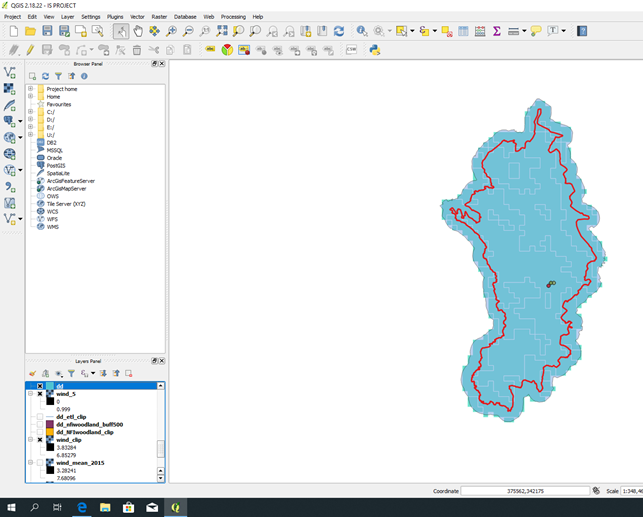
\includegraphics[width=0.6\textwidth]{figures/vectorization}
 \caption{Vectorización en QGIS.}
 \label{fig:vectorization}
\end{figure}

% =====================================================================
\section{Resultados y discusión}

\subsection{Mapas temáticos}
La Figura~\ref{fig:dndvi} muestra que la mayor parte de la ROI presenta valores de $\Delta$NDVI cercanos a cero, como se espera para bosques y pastos estables entre dos fechas separadas solo 25 días. Las anomalías negativas fuertes se concentran en las paredes empinadas del cañón alto del río Ingará (sector noroccidental, alrededor de La Italia) y en las laderas y vías que rodean a San José del Palmar, y coinciden con las nuevas cicatrices de color marrón claro visibles en el compuesto en color verdadero de $t_2$ (Figura~\ref{fig:t2tc}). El mapa de $\Delta$NIR (Figura~\ref{fig:dnir}) confirma el mismo patrón. La Figura~\ref{fig:landslides} muestra los polígonos finales de deslizamientos, y la Figura~\ref{fig:zoom} amplía el conglomerado más grande, donde las laderas con bosque y pastos al norte del río Ingará en $t_1$ aparecen en $t_2$ como cicatrices frescas de suelo desnudo, coincidiendo exactamente con los polígonos y con los valores más fuertes de $\Delta$NDVI ($< -0.4$). Algunas manchas de $\Delta$NDVI positivo (verde) cerca de San José del Palmar corresponden a áreas afectadas por sombra de nube o bruma en $t_1$ que la SCL no capturó por completo, y a rebrote de cultivos; no afectan la detección de pérdidas.

\fig{fig_landslides.jpg}{Deslizamientos cosísmicos detectados (contornos rojos) sobre el compuesto en color verdadero de $t_2$.}{fig:landslides}
\fig[1.0]{fig_zoom_largest.jpg}{Ampliación del conglomerado de deslizamientos más grande (cañón alto del río Ingará): $t_1$ (izquierda), $t_2$ con los polígonos detectados (centro) y $\Delta$NDVI (derecha).}{fig:zoom}

\subsection{Estadísticas}
\begin{table}[H]
    \centering
    \caption{Resumen estadístico de la detección de cambios.}
    \label{tab:stats}
    \begin{tabular}{lr}
        \toprule
        \textbf{Métrica} & \textbf{Valor} \\
        \midrule
        Área de la ROI & 49.7 km$^2$ \\
        Área válida (sin nubes) & 95.2\% \\
        Media $\mu$ / desviación estándar $\sigma$ del $\Delta$NDVI & $-0.0075$ / $0.0467$ \\
        Umbral $\mu - 2\sigma$ & $-0.101$ \\
        Número de polígonos de deslizamiento & 181 \\
        Área total de deslizamientos & 95.2 ha (0.95 km$^2$) \\
        Polígono mayor / medio / mediana & 6.03 / 0.53 / 0.23 ha \\
        Porcentaje de la ROI afectado & 1.9\% \\
        \midrule
        $\Delta$NDVI medio dentro de los deslizamientos & $-0.18$ \\
        NDVI medio dentro de los deslizamientos ($t_1 \rightarrow t_2$) & $0.81 \rightarrow 0.63$ \\
        Polígonos por tamaño (0.1--0.5 / 0.5--1 / 1--5 / $\geq$5 ha) & 135 / 19 / 25 / 2 \\
        \bottomrule
    \end{tabular}
\end{table}

\subsection{Narrativa y discusión}
El patrón espacial de los cambios detectados es coherente con el contexto físico del evento. La profundidad intermedia del sismo ($\sim$110~km) distribuyó la sacudida fuerte sobre una región amplia en lugar de concentrarla junto al epicentro; en las laderas empinadas, profundamente meteorizadas y saturadas por la lluvia de la Cordillera Occidental, esa sacudida bastó para detonar numerosos deslizamientos superficiales. El cañón del río Ingará, con sus laderas convexas y cortes de vía, es precisamente donde se agrupan las anomalías de $\Delta$NDVI. Estas fallas bloquearon las vías que comunican a San José del Palmar con el Eje Cafetero, lo que explica por qué el municipio, uno de los más aislados del Chocó, permaneció incomunicado durante los primeros días de la emergencia, dificultando las labores de rescate y abastecimiento.

La región tiene una larga historia de sismos dañinos de profundidad intermedia, como los eventos de 1979 y 1995 que afectaron al Eje Cafetero; el evento de 2026 muestra nuevamente que la amenaza sísmica y la amenaza por deslizamientos en la Cordillera Occidental deben considerarse de forma conjunta en el ordenamiento territorial, en especial para los corredores viales y los asentamientos rurales en ladera.

\textbf{Limitaciones.} (i) La nubosidad persistente limitó la elección de fechas y redujo el área analizable; (ii) el $\Delta$NDVI también puede capturar pérdidas de vegetación no sísmicas (cosechas, talas, quemas), lo que se reducirá en la entrega final con un filtro de pendiente derivado del DEM de Copernicus; (iii) la resolución de 10~m no resuelve deslizamientos menores a $\sim$0.1~ha; (iv) es posible que aún no existan imágenes de muy alta resolución posteriores al evento en Google Earth para la validación. Se propone Sentinel-1 SAR (no afectado por las nubes) como complemento para el componente de daño urbano en Pereira.

% =====================================================================
\section{Conclusiones}
Se implementó un flujo de trabajo bitemporal reproducible, basado en datos gratuitos Sentinel-2 L2A y software libre (QGIS), para cartografiar los deslizamientos cosísmicos del sismo $M_w$~7.4 del 10 de agosto de 2026 alrededor de San José del Palmar. Un preprocesamiento cuidadoso (reflectancia BOA, grilla común de 10~m en EPSG:9377 y enmascaramiento de nubes con la SCL) hizo que las dos fechas fueran radiométrica y geométricamente comparables, de modo que las diferencias de $\Delta$NDVI y $\Delta$NIR reflejan cambios reales en la superficie. El umbral estadístico ($\mu - 2\sigma$) y la vectorización identificaron 181 polígonos de deslizamiento que suman 95.2~ha (1.9\%) en un área de 49.7~km$^2$; la mayoría son fallas superficiales pequeñas ($<$0.5~ha), con algunos deslizamientos grandes de hasta 6~ha concentrados en el cañón alto del río Ingará. La siguiente etapa incorporará un filtro de pendiente, una clasificación supervisada con matriz de cambio \emph{De-A} (\emph{From-To}) y una evaluación formal de la exactitud (matriz de confusión, Kappa y F1-score).

\printbibliography[title={Referencias}]

\end{document}
